% THIS IS SIGPROC-SP.TEX - VERSION 3.1
% WORKS WITH V3.2SP OF ACM_PROC_ARTICLE-SP.CLS
% APRIL 2009
%
% It is an example file showing how to use the 'acm_proc_article-sp.cls' V3.2SP
% LaTeX2e document class file for Conference Proceedings submissions.
% ----------------------------------------------------------------------------------------------------------------
% This .tex file (and associated .cls V3.2SP) *DOES NOT* produce:
%       1) The Permission Statement
%       2) The Conference (location) Info information
%       3) The Copyright Line with ACM data
%       4) Page numbering
% ---------------------------------------------------------------------------------------------------------------
% It is an example which *does* use the .bib file (from which the .bbl file
% is produced).
% REMEMBER HOWEVER: After having produced the .bbl file,
% and prior to final submission,
% you need to 'insert'  your .bbl file into your source .tex file so as to provide
% ONE 'self-contained' source file.
%
% Questions regarding SIGS should be sent to
% Adrienne Griscti ---> griscti@acm.org
%
% Questions/suggestions regarding the guidelines, .tex and .cls files, etc. to
% Gerald Murray ---> murray@hq.acm.org
%
% For tracking purposes - this is V3.1SP - APRIL 2009

\documentclass{acm_proc_article-sp}

\usepackage{caption}
\usepackage{soul}
\usepackage{color}
\usepackage{url}
\usepackage{hyperref}
\usepackage{subfig}
\usepackage{graphicx}
%\usepackage{algpseudocode}

\begin{document}
\title{Evaluating BLAST Results}
\subtitle{Assignment 7}
%
% You need the command \numberofauthors to handle the 'placement
% and alignment' of the authors beneath the title.
%
% For aesthetic reasons, we recommend 'three authors at a time'
% i.e. three 'name/affiliation blocks' be placed beneath the title.
%
% NOTE: You are NOT restricted in how many 'rows' of
% "name/affiliations" may appear. We just ask that you restrict
% the number of 'columns' to three.
%
% Because of the available 'opening page real-estate'
% we ask you to refrain from putting more than six authors
% (two rows with three columns) beneath the article title.
% More than six makes the first-page appear very cluttered indeed.
%
% Use the \alignauthor commands to handle the names
% and affiliations for an 'aesthetic maximum' of six authors.
% Add names, affiliations, addresses for
% the seventh etc. author(s) as the argument for the
% \additionalauthors command.
% These 'additional authors' will be output/set for you
% without further effort on your part as the last section in
% the body of your article BEFORE References or any Appendices.

%\numberofauthors{3} %  in this sample file, there are a *total*
% of EIGHT authors. SIX appear on the 'first-page' (for formatting
% reasons) and the remaining two appear in the \additionalauthors section.
%
\numberofauthors{1}
\author{
	\alignauthor Caitlin Ross\\
	\affaddr{Computer Science Department, Rensselaer Polytechnic Institute} \\
	\email{rossc3@rpi.edu}
}
% There's nothing stopping you putting the seventh, eighth, etc.
% author on the opening page (as the 'third row') but we ask,
% for aesthetic reasons that you place these 'additional authors'
% in the \additional authors block, viz.

\date{30 July 1999}
% Just remember to make sure that the TOTAL number of authors
% is the number that will appear on the first page PLUS the
% number that will appear in the \additionalauthors section.

\maketitle

\begin{abstract}
Here I run a given DNA sequence through nucleotide BLAST.  I report some basic information for the top ten results, as well as some more detailed information for the highest match found with BLAST.  The given DNA sequence is a match for the gene coding sequence for casein kinase 1 in Plasmodium falciparum, a parasite responsible for causing malaria in humans.  

\end{abstract}


\section{Problem Statement}
I was given a fasta file with a DNA sequence.  The problem here is to run this sequence through BLAST, report the top 10 results, and do some research on the species the sequence belongs to.


\section{Results}
As my Ross.fasta file contained a DNA sequence, I used nucleotide BLAST to run on the sequence. The top 10 results from BLAST are shown:

\begin{enumerate}
 \item \textit{Plasmodium falciparum} 3D7 casein kinase 1, PfCK1 (PfCK1) mRNA, complete cds \\
 match length: 1207 \\
 e-value: 0.0 \\
 bit-score: 828 \\
 \% identity: 100\% \\
 strand: Plus/Plus \\
 
 \item \textit{Plasmodium falciparum} casein kinase 1 (CK1) mRNA, complete cds \\
  match length:1297  \\
 e-value: 0.0 \\
 bit-score: 817 \\
 \% identity: 99\%\\
 strand: Plus/Plus \\
 
 \item \textit{Plasmodium reichenowi} casein kinase 1 (CK1), partial mRNA \\
  match length: 972 \\
 e-value: 0.0 \\
 bit-score: 767 \\
 \% identity: 99\% \\
 strand: Plus/Plus \\
 
 \item \textit{Plasmodium berghei} strain ANKA casein kinase 1 (PB000530.02.0), partial mRNA \\
  match length: 735 \\
 e-value: 1e-149 \\
 bit-score: 540 \\
 \% identity: 89\% \\
 strand: Plus/Plus \\
 
 \item \textit{Plasmodium yoelii yoelii} str. 17XNL casein kinase i (PY06011) partial mRNA \\
  match length: 972 \\
 e-value: 5e-148 \\
 bit-score: 534 \\
 \% identity: 89\% \\
 strand: Plus/Plus \\
 
 \item \textit{Plasmodium vinckei vinckei} CK1/CK1 protein kinase partial mRNA \\
  match length: 972 \\
 e-value: 5e-143 \\
 bit-score: 518 \\
 \% identity: 89\%\\
 strand: Plus/Plus \\
 
 \item \textit{Plasmodium berghei} strain ANKA hypothetical protein (PB300304.00.0) partial mRNA \\ 
  match length: 549 \\
 e-value: 9e-81 \\
 bit-score: 311 \\
 \% identity: 90\% \\
 strand: Plus/Plus \\
 
 \item \textit{Plasmodium chabaudi chabaudi} casein kinase 1 (PC000102.03.0) partial mRNA \\
  match length: 540 \\
 e-value: 1e-79 \\
 bit-score: 307 \\
 \% identity: 91\% \\
 strand: Plus/Plus \\
 
 \item \textit{Plasmodium falciparum} 3D7 chromosome 11, complete sequence \\
  match length: 2038337 \\
 e-value: 9e-71 \\
 bit-score: 278 \\
 \% identity: 99\% \\
 strand: Plus/Minus \\
 
 \item \textit{Plasmodium yoelii} genome assembly PY17X01, chromosome : 9 \\
  match length: 1824586 \\
 e-value: 2e-22 \\
 bit-score: 117 \\
 \% identity: 95\% \\
 strand: Plus/Plus \\
 
\end{enumerate}
BLAST reports that the highest match for the given DNA sequence is ``\textit{Plasmodium falciparum} 3D7 casein kinase 1, PfCK1 (PfCK1) mRNA, complete cds.''  The alignment for this match is shown in Figure 1.  This match reports that the sequence is the coding DNA sequence (CDS) for the casein kinase 1 for the protozoan (unicellular eukaryote) \textit{Plasmodium falciparum}.  Genes are composed of introns and exons.  Introns are spliced out and the remaining exons make up the CDS.  

Kinases are enzymes that phophorylate proteins and specifically, the casein kinase 1 is an enzyme that regulates signal transduction pathways in many eukaryotic cells\footnote{\url{https://en.wikipedia.org/wiki/Kinase}}.  Casein kinases appear to be important to activities such as circadian rhythm, DNA repair, and DNA transcription\footnote{\url{https://en.wikipedia.org/wiki/Casein_kinase_1}}.  

The match is found in the species \textit{Plasmodium falciparum}.  \textit{P. falciparum} is a parasite that is transmitted by mosquitos and causes the most dangerous form of malaria\footnote{\url{https://en.wikipedia.org/wiki/Plasmodium_falciparum}}.  

\begin{figure}[!b]
	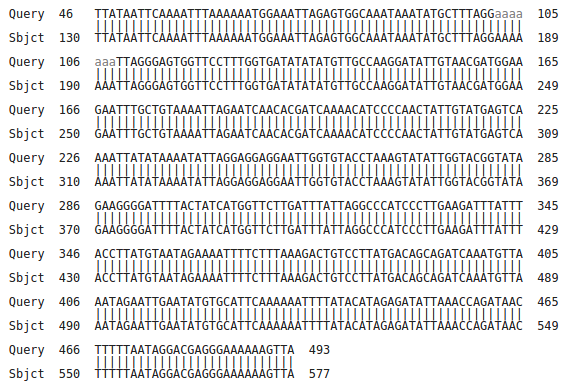
\includegraphics[trim={0 0 2cm 0}, clip,width=3.5in]{alignment-cropped.png}
	\caption{BLAST alignment for the highest match}
	\label{fig:hist}
\end{figure}

  
%
% The following two commands are all you need in the
% initial runs of your .tex file to
% produce the bibliography for the citations in your paper.
\bibliographystyle{abbrv}
%\bibliography{sigproc}  % sigproc.bib is the name of the Bibliography in this case

% You must have a proper ".bib" file
%  and remember to run:
% latex bibtex latex latex
% to resolve all references
%
% ACM needs 'a single self-contained file'!
%
%APPENDICES are optional
%\balancecolumns

\balancecolumns
% That's all folks!
\end{document}
